% AOSD report template
% Valentino Vranić 2018

\documentclass[11pt,english,a4paper,twoside]{article}
%\documentclass[11pt,slovak,a4paper,twoside]{article}

\usepackage[IL2]{fontenc}

\usepackage[utf8]{inputenc}
\usepackage{babel}
\usepackage{url}
\usepackage[nottoc]{tocbibind}
\usepackage{ifthen}
\usepackage[hidelinks]{hyperref}
\usepackage{graphicx}
\usepackage{listings}
\usepackage{verbatim}
\usepackage{float}
\lstset{language=[AspectJ]Java,basicstyle=\fontsize{9}{10.8}\selectfont,showstringspaces=false,columns=fullflexible}

\newcommand{\magnf}{.65}
\newcommand{\codesize}{\footnotesize}
\newcommand{\lsti}{\ajset\lstinline[basicstyle=\fontsize{10}{12}\selectfont]}
\newcommand{\emp}[1]{\emph{#1}}
\newcommand{\ffe}[1]{\textsf{#1}}

% balík listings niekedy niektoré kľúčové slová nezvýrazňuje ak to nedostane príkazom tesne pred textom
\newcommand{\ajset}{\lstset{emph={class,aspect,new,call,execution,set,int,advice,public,thisJoinPointStaticPart,thisEnclosingJoinPointStaticPart,@annotation,dominates},emphstyle=\bfseries}}

\newcommand{\reporttitle}{Data versioning in machine-learning architecture}
% here goes your fancy title

\pagestyle{myheadings}
\markboth{\reporttitle}{Software Architecture 2024/25, FIIT STU}

\title{\reporttitle}

\author{Peter Bartoš, Stanislav Krištof} % your name

\date{Faculty of Informatics and Information Technologies\\
      Slovak University of Technology in Bratislava\\[6pt]
      \today}



\begin{document}

\maketitle

\begin{abstract}
Data versioning plays a crucial role in modern machine learning architecture,
ensuring that the complex and ever-evolving datasets that provide the basis for
models can be tracked, compared, and managed efficiently. At its core, data
versioning refers to the practice of creating unique references for different
states of a dataset over time, allowing us to trace changes, restore previous
versions, and debug issues. This is vital in machine learning workflows, where
even small changes in data can significantly impact model performance.

In this domain, data versioning supports reproducibility by maintaining a
consistent link between datasets and the models trained on them. Without version
control, it becomes challenging to recreate experiments, leading to
inconsistencies in predictions and hindering model audits. Versioning also
simplifies collaboration across teams, enabling multiple stakeholders to work on
the same data without overwriting each other's progress.

Basic approaches to data versioning systems (DVS) include full duplication of
datasets, where copies are saved with each change, and metadata-based
versioning, where timestamps indicate the validity of each record. Advanced
solutions (like lakeFS and DVC) deal with versioning as a core component of
machine learning architecture. They enable storage-efficient data commits,
branching, and comparison, similar to how Git handles version control in
software development.

Overall, data versioning enhances productivity, reduces errors, and fosters an
engineering-driven approach to handling data in machine learning pipelines,
ultimately enabling smoother transitions between development stages and more
robust model deployment. The objective of the project is to go over these
systems and provide detailed overviews of how data versioning has such a crucial
role in machine learning architecture.
\end{abstract}


\section{Introduction} \label{in}

Reproducibility, as defined by ACM \cite{ACMreproducibility}, 
is the ability to obtain precise measurements by different 
teams under the same conditions. In AI advancements, reproducibility 
is crucial, with Peng \cite{peng2011reproducible} considering it 
the ultimate measure of scientific validity. However, Pawlik et 
al. \cite{pawlik2019link} found that only 7.64\% of analyzed papers 
were reproducible. Improved data version control can enhance 
reproducibility and enable more complex studies, increasing understanding 
of neural networks. Pawlik et al. \cite{pawlik2019link} suggest that 
datasets should include not only input data but also raw data and 
preparation instructions to improve context and reproducibility. 
\\\\
To understand how data versioning integrates into machine learning 
architecture, it's essential to examine key components and workflows. 
Machine learning pipelines rely on iterative experimentation, where 
data is critical at every stage, from preprocessing to model training, 
evaluation, and deployment. Maintaining consistent, traceable versions 
of datasets and models is vital for ensuring reproducibility. 
\cite{wandb}

\section{Version control in Machine Learning} \label{intro2ml}
In the process of developing a machine learning model, 
various artifacts beyond source code are produced. An 
artifact refers to any file that serves as an input or 
output of a given process. In traditional software 
development, inputs such as source code and libraries 
qualify as artifacts, while outputs like object files 
and executables are also considered artifacts. For 
instance, in a build process, these outputs represent 
the results of transforming inputs through the 
compilation pipeline. \cite{wandb, pulicharla2024data}

In the context of machine learning, the most critical 
artifacts are datasets and models. Datasets act as the 
inputs to the training process, while models, which 
encapsulate learned parameters and structures, serve as 
the outputs of this process. \cite{pulicharla2024data}
\begin{figure}[H]
    \centering
    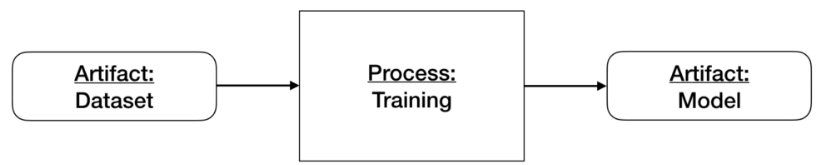
\includegraphics[width=0.8\textwidth]{fig/ml-artifacts.png}
    \caption{Artifacts in Machine Learning \cite{wandb}}
    \label{fig:ml-artifacts}
\end{figure}

\subsection{Use of Data Versioning in Machine Learning}

In machine learning workflows, managing datasets is as important 
as managing code, especially when it comes to reproducibility and 
collaboration. A systematic approach to data versioning enables 
teams to track, store, retrieve, and switch between different 
versions of datasets seamlessly, ensuring consistency across 
development and experimentation phases. \cite{wandb, pulicharla2024data}
\\\\
The process begins with versioning the dataset. Just as changes 
in source code are tracked, datasets need to be tracked too. 
Metadata files can be created to store information about each 
dataset version without including the actual dataset itself, 
keeping the repository efficient. These metadata files act as 
pointers to the specific dataset version associated with a 
particular stage of the machine learning pipeline. 
\cite{pulicharla2024data, opendatascience}
\\\\
Next, the dataset itself is stored in a dedicated storage 
system. This storage can be local or cloud-based, and it holds 
the actual data files. By separating the data from the metadata 
stored in the repository, teams can handle large datasets without 
bloating their version control systems, while still ensuring that 
every version is accounted for.\cite{opendatascience}
\\\\
Retrieving a specific dataset version is then made possible 
through the metadata file. The system can fetch the corresponding 
dataset version from storage based on the metadata, ensuring 
that the data matches the state of the code and experiments 
conducted at that time. This eliminates ambiguity and enhances 
reproducibility in experiments. \cite{opendatascience, yizhenzhao}
\\\\
Lastly, the ability to switch between dataset versions ensures 
flexibility during development. Just as a developer can revert 
to an earlier version of their code, they can also revert to or 
load the dataset version that was used with that code. This 
synchronization between code and data allows for iterative 
testing, analysis, and debugging, supporting more rigorous and 
reproducible experimentation. \cite{opendatascience, yizhenzhao}
\\\\
By implementing data versioning practices in this way, teams 
can ensure that their machine learning workflows are robust, 
efficient, and conducive to collaboration, enabling seamless 
transitions across different stages of development and research.
\cite{wandb, opendatascience, yizhenzhao}

\begin{figure}[H]
    \centering
    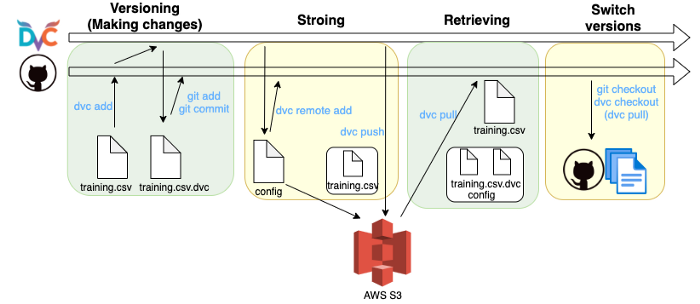
\includegraphics[width=0.8\textwidth]{fig/ml-dv-example.png}
    \caption{Example of how can be data versioning used in 
    machine learning (DVC and GIT as examples) \cite{opendatascience}}
    \label{fig:ml-dv-example}
\end{figure}

\subsection{Advantages of Data Versioning in Machine Learning}

In machine learning workflows, data versioning is not just 
about tracking changes; it also facilitates collaboration 
across multiple teams and ensures consistency in model 
development processes. By creating a structured system of 
versioning, practitioners can manage datasets and models at 
different stages of development, allowing seamless integration, 
testing, and improvement of machine learning pipelines.
\cite{wandb, opendatascience}
\\\\
Data versioning enables branching and merging of datasets, 
similar to how code branches work in software development. This 
is especially important when multiple teams or practitioners work 
on different aspects of a project. For instance, different projects 
or teams may use the same foundational dataset but modify or enhance 
it according to specific needs. These changes can be organized 
into separate "streams" or versions, ensuring that each team 
has a clear record of its modifications while still maintaining 
a connection to the original data.
\cite{wandb, opendatascience}
\\\\
Versioning also allows for "harvesting", where changes or 
improvements made in one branch can be integrated back into the 
main dataset or shared across other streams. This ensures that 
advancements in one area can benefit the broader workflow 
without disrupting other teams' progress. Similarly, the 
propagation of changes ensures consistency across different 
projects and keeps all streams aligned with the latest updates.
\cite{opendatascience, aimultiple}
\\\\
Moreover, data versioning systems can track multiple 
hierarchical streams, ranging from enterprise-level datasets 
to project-specific and even individual practitioners' 
workstreams. This hierarchical structure ensures flexibility 
and scalability, allowing datasets to evolve alongside their 
respective machine learning models.
\cite{opendatascience, aimultiple}
\\\\
By implementing a robust data versioning framework, teams can 
manage data lineage, collaborate effectively, and ensure 
reproducibility, even in complex machine learning ecosystems. 
This structured approach enhances the ability to build, test, 
and deploy models with greater confidence.
\cite{opendatascience, aimultiple}

\begin{figure}[H]
    \centering
    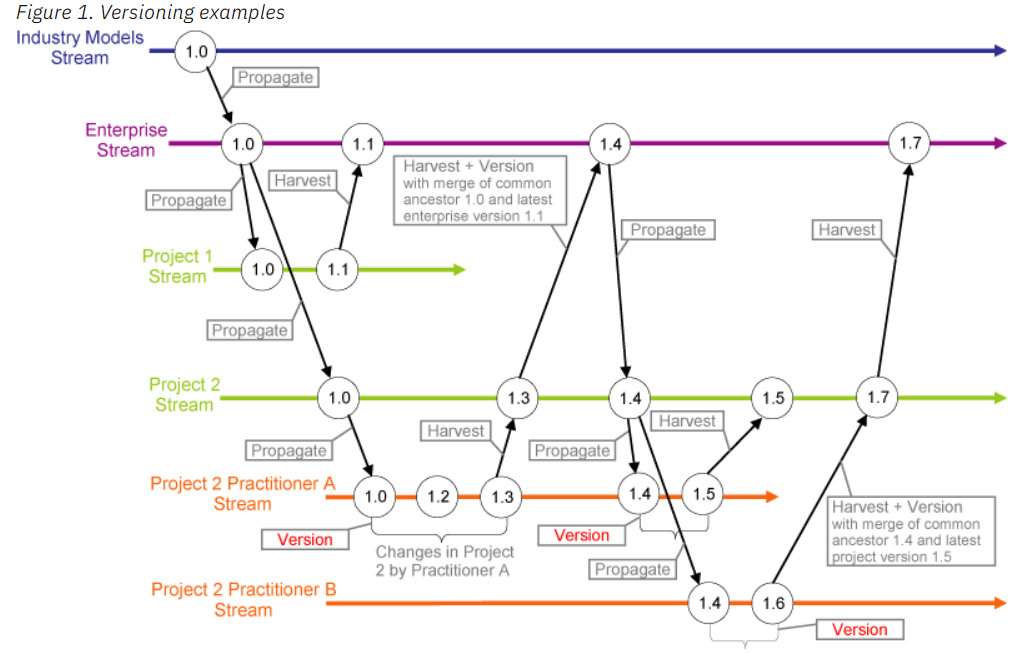
\includegraphics[width=0.8\textwidth]{fig/dv-advantages.png}
    \caption{An example of hierarchical data versioning 
        streams showcasing branching, propagation, and 
        merging across industry, enterprise, project, and 
        individual practitioner levels, enabling collaborative 
        and scalable data management in machine learning 
        workflows \cite{aimultiple}}
    \label{fig:dv-advantages}
\end{figure}


% tu by som zmenil názov na niečo také ako state of the art 
% alebo niečo také, lebo tu popisuješ vlastne, že aké 
% technológie sa teraz na to používajú
\section{Insight into\ldots} \label{insight}
\paragraph{Types of Data Version Control Systems (DVCS)}
According to Zolkifli et al. \cite{zolkifli2018version} in centralised DVCS, a
singular repository is located on the server. These DVCS are suitable for teams
with smaller number of members, with the team being located in a single place.
Only the last version of a file is retrieved and there is a single point of
failure. Examples include Apache Subversion or Perforce Revision Control System.
In distributed DVCS, on the other hand, each user has one local repository.
Examples include Git, Mercurial, Bazaar or Bitkeeper. This type is suitable
regardless of team size. It also enables users being located in different parts
of the world. Clients can create their own branches and sync them with the
server.
\paragraph{Git}
As stated by Komsiyski \cite{komsiyski2013binary}, Git works on basis of patch
files. As noted by Bryan \cite{bryan2018excuse}, large and often changing files
are not suitable for Git, since they can slow down pushes and pulls. According
to Perez et al. \cite{perez2016ten}, binary files in git are stored as a single
large entity. Therefore, even small changes lead to new copies in the
repository. This also makes it difficult to compare changes in files using diff
and may lead to frequent merge conflicts.

\paragraph{Git LFS}
Git also offers an extension for large files called Git LFS (Large File
Storage), which enables more efficient handling of large files
\cite{perez2016ten}. Content of the file is stored in cloud, with the repository
containing only pointers to the files, as noted in the documentation
\cite{gitlfs-structure} (Figure \ref{fig:gitlfs-architecture}). Since Git LFS is
a GitHub extension, its advantages are compatibility with Git
\cite{gitlfs-collaboration} and file agnosticism (compatibility with all file
formats) \cite{comparison}. Its disadvantages are inefficient storage management
- similar to Git, edited files are stored as new files. Therefore, it is not
suitable for large frequently-changing files, especially if they are compressed
(such as file formats frequently used in computer vision, e.g. jpg, png)
\cite{git-lfs}. In addition, data in Git LFS do not stay in place. It also does
not scale as well and its data retrieval is slow. As such, this approach is
suitable mostly for game developers and not for for ML and data science
purposes.

\begin{figure}[H]
    \centering
    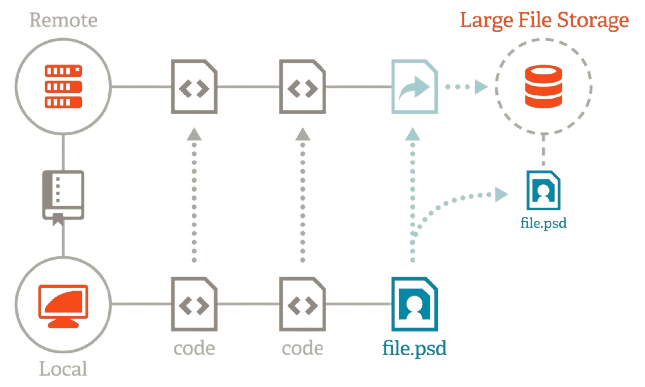
\includegraphics[width=0.8\textwidth]{fig/gitlfs-arch.png}
    \caption{Software architecture of Git LFS \cite{gitlfs-architecture}}
    \label{fig:gitlfs-architecture}
\end{figure}

\begin{comment}
Git offers a Large File Storage (LFS) module that
replaces such large files with pointers while the large binary file can be
stored remotely, which results in smaller and faster repositories. Git LFS is
also supported by GitHub, albeit with a space quota or for a fee, to retain your
usual GitHub workflow (https://help.github.com/categories/managing-large-files/)
(S1 File, Section 1).

GIT LFS (Large File Storage)

files above 50mb should be commited using Git LFS. 1 GiB of storage is free for
every account, together with 1GiB bandwidth. 5$ = 50 GiB storage, 50 GiB
bandwidth. text pointers are stored in git, the actual binary files are on cloud


https://www.atlassian.com/git/tutorials/git-lfs
https://docs.github.com/en/repositories/working-with-files/managing-large-files/about-storage-and-bandwidth-usage

When you commit and push a change to a file tracked with Git LFS, a new version
of the entire file is pushed and the total file size is counted against the
repository owner's storage limit. When you download a file tracked with Git LFS,
the total file size is counted against the repository owner's bandwidth limit.
Git LFS uploads do not count against the bandwidth limit.

For example:

If you push a 500 MB file to Git LFS, you'll use 500 MB of your allotted storage
and none of your bandwidth. If you make a 1 byte change and push the file again,
you'll use another 500 MB of storage and no bandwidth, bringing your total usage
for these two pushes to 1 GB of storage and zero bandwidth. If you download a
500 MB file that's tracked with LFS, you'll use 500 MB of the repository owner's
allotted bandwidth. If a collaborator pushes a change to the file and you pull
the new version to your local repository, you'll use another 500 MB of
bandwidth, bringing the total usage for these two downloads to 1 GB of
bandwidth. If GitHub Actions downloads a 500 MB file that is tracked with LFS,
it will use 500 MB of the repository owner's allotted bandwidth.
git works on basis of patch files, as Komsiyski states

\cite{komsiyski2013binary}, time for creating a patch and sending the patch to a
server has to be less than the time needed to send a new version of file to the
server.
\end{comment}
\paragraph{Dolt}
Dolt is a version-controlled SQL database and as such it may serve as an example
of a centralised DVS. Analogous to Git, one can track schemas and changes in the
database, create and merge branches \cite{dolt-reproducibility}. Under the hood,
Dolt uses Prolly trees - a data structure related to both B-trees
\cite{prolly-trees}, commonly used in RDBMS and Merkle trees (used by
distributed version control systems such as Git or Mercurial)\cite{comparison}.
This data structure provides both fast performance (including diffs and merges)
and efficient storage management (each portion of data shared between trees is
shared only once). However, like other RDBMS, while Dolt may be the ideal
solution for structured data, it is not suitable for unstructed data.
\begin{comment}
    version controlled SQL DB; suitable for data stored in RDBMS (such as MySQL,
although there appears to be a postgres version as well) usage of prolly trees
(merge of B-tree (indices of RDBMS, performance of databases) and Merkle tree
(structure used in git)) = data is saved in accordance to hash (easier
identification whether file changed, better diff / merge);not suitable for
unstructured data, nor high performance; centralised; tracking of schemas and
changes in the database ;(source: github read me file);
https://docs.dolthub.com/introduction/use-cases = overview of usecases not great
for unstructured binary files; can effectively serve to replace databases;
support merging, branching and other typical git stuff;
\end{comment}
\paragraph{DVC by Iterative}
Another solution, suitable for ML learning may be DVC \cite{DVC}. DVC achieves
faster data retrieval by its data staying in place. In addition, DVC also uses a
caching layer (Figure \ref{fig:dvc-architecure}), which allows faster data
retrieval for multiple members of team \cite{comparison}. DVC supports both
structured and unstructed data. It however does not support RDBMS. Since it
caters to data scientists, it offers several features which greatly lead to
higher reproducibility, such as defining data pipelines
\cite{dvc-define-pipelines}, visualisation of pipelines
\cite{dvc-run-pipelines}, experiment tracking \cite{dvc-compare-experiments} and
hydra compatibility \cite{dvc-hydra}. It also does not scale as well, mostly due
to the same reasons as git.

\begin{figure}[H]
    \centering
    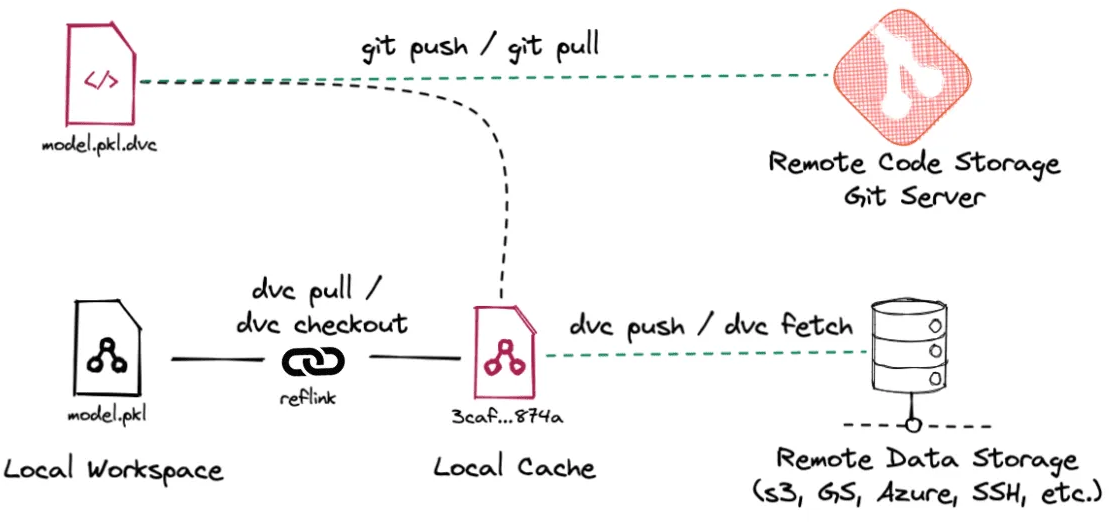
\includegraphics[width=0.8\textwidth]{fig/dvc-arch.png}
    \caption{Software architecture of DVC \cite{comparison}}
    \label{fig:dvc-architecture}
\end{figure}

\begin{comment}
Iterative offers DVC \cite{DVC}, which allows users to save and track model data
and models. Data and models are captured using git commits and can be stored
both locally or in cloud. DVC works by creating metafiles, that describe data to
be tracked. metafiles are put in Git instead of large files.
\end{comment}

\section{Conclusions and Further Work} \label{cc}
Data versioning has proven to be an indispensable 
component of modern machine learning workflows, 
addressing critical challenges such as reproducibility, 
collaboration, and scalability. As demonstrated, implementing 
data versioning systems (DVS) enables teams to track and 
manage datasets efficiently, ensuring consistency and 
traceability throughout the machine learning pipeline. 
The discussion on tools like Git LFS, Dolt, and DVC 
highlights the varying approaches to tackling version 
control, emphasizing the trade-offs between structured 
and unstructured data management, performance, and scalability.


Despite these advancements, challenges remain. Centralized 
systems often struggle with scalability and single points of 
failure, while distributed systems require efficient handling 
of large, frequently changing datasets. Tools like Git LFS, 
although widely used, are limited in their capacity to manage 
large binary files effectively. Similarly, while Dolt is 
highly efficient for structured data, it does not address 
unstructured data needs. DVC offers significant advantages 
for data scientists but lacks support for relational database 
management systems (RDBMS).

Future research and development in data versioning would focus 
on developing systems that can efficiently handle large, 
frequently updated datasets, especially those used in 
domains like computer vision, genomics, and IoT. 
There is also a need to address the designing of hybrid 
systems that can seamlessly manage both relational and 
non-relational data to address the diverse needs of modern 
machine learning workflows. Also leveraging AI to 
automate dataset versioning is also a must. This would 
identify anomalies, and suggest optimal data branches or 
merges based on usage patterns. For final touches there needs 
to be a better performance optimization to ensure faster 
data retrieval, reduced storage overheads, and better 
handling of binary files through innovations in data 
structures and caching mechanisms. 

By addressing these challenges, data versioning systems can 
continue to evolve, further cementing their role as a 
foundational element of machine learning architecture. 
In doing so, they will not only improve the efficiency and 
reliability of machine learning pipelines but also unlock new 
possibilities for reproducibility and collaboration in the 
broader AI and data science community.


\bibliographystyle{abbrv} % plain or alpha are fine, too
\bibliography{bib}


\end{document}

